\section{Declaration of Generative AI Use}
\label{app:ai_declaration}
During the preparation of this project and report, the authors used generative AI tools---specifically GPT~6, Fable~5.2, Opus~5.5, and Gemini~4 (Carbon, Argon, Neon, and Hydrogen)---for discovering and summarizing relevant literature, English language polishing, LaTeX formatting, and assisting with drafting, refactoring, and debugging auxiliary engineering, Slurm, data-processing, and visualization scripts. All core research ideas, experimental designs, analyses, and scientific conclusions are the authors' own work. Every AI-assisted code snippet, text revision, and literature reference was critically reviewed, tested, and verified by the authors against primary sources, and all reported results and figures originate strictly from real experiments conducted by the team on the NUS SoC compute cluster. The authors take full responsibility for the content, accuracy, and academic integrity of this submission.

\section{Implementation Details and Code Reproducibility}
\label{app:impl}
All code, Slurm scripts, environment definitions, and result summaries are publicly available at \url{https://github.com/ziyouledi/CS5478_project} (see repository \texttt{README.md} and \texttt{Experiment Plan/cluster\_smoke/README.md} for end-to-end reproduction instructions).

\paragraph{Runtime and hardware.}
Simulation and RL runs use Isaac Lab v2.3.1 (commit \texttt{5c2ec81c}), Isaac Sim 5.1.0.0, Python 3.11.17, PyTorch 2.7.0+cu128, and RL-Games 1.6.1 on NUS SoC Slurm GPU nodes (NVIDIA Tesla T4 15~GB for 2,048-env training/evaluation; NVIDIA H200 141~GB for 8,192-env \texttt{Unified v4} training).
VLM inference and LoRA training run on NVIDIA H100 (47/96~GB) using vLLM 0.11.0, PyTorch 2.8.0, and Transformers 4.57.6.

\paragraph{PPO and asymmetric critic hyperparameters.}
All Stage 1, M1, M2, and rate-sweep PPO runs train for 5,000 iterations with 2,048 parallel environments (163.84M transitions, horizon 16, minibatch 32,768, 5 mini-epochs, adaptive learning rate $5\times 10^{-4}$, target KL 0.016, actor MLP \texttt{[512, 512, 256, 128]} with ELU).
In goal-hidden stages (M1, M2-hidden, E1, E3), the 8 goal observation entries \texttt{obs[64:72]} (\texttt{goal\_rot} and \texttt{quat\_mul(object\_rot, conj(goal\_rot))}) are removed from the actor while \texttt{central\_value\_config} receives the full clipped 157-D state with matching network architecture, minibatch size, and 5 mini-epochs.
Frozen experts are verified by SHA-256 checksums before every rollout and student run; all learning curves evaluate 25 checkpoints (every 200 iterations) over 1,024 deterministic episodes.

\section{Stage 1 (Goal-Visible) Results and Spectral Diagnostics}
\label{app:stage1}
Table~\ref{tab:app_stage1} summarizes Stage 1 goal-visible learning efficiency on Task 1 (21 runs, $P_E=26.11$) and Task 2 M2 (30 runs including \texttt{joint-2/4}, $P_E=31.14$).
When the actor observes the goal directly, no intent condition differs significantly from \texttt{blind} (Task 1 one-way ANOVA N80 $p=0.82$, AUC $p=0.65$; Task 2 ANOVA N80 $p=0.90$, AUC $p=0.82$, final $p=0.69$; with a 4th seed on \texttt{blind}/\texttt{hand-2}/\texttt{joint-2}, \texttt{hand-2} vs.\ \texttt{blind} AUC Welch $p=0.060$ remains non-significant).
On Task 2, \texttt{joint-$k$} (projecting expert actions onto the joint-position PCA basis) captures less action variance than action PCA (38.1\% vs.\ 42.7\% at $k=2$; 55.9\% vs.\ 64.0\% at $k=4$) and does not outperform \texttt{hand-$k$}.
Diagnostic PCA on measured 24-D joint positions on Task~1 confirms that high dimensionality is intrinsic rather than a bang-bang artifact: joint positions are much smoother (6.2\% at limits vs.\ 62.2\% for actions; 5.2\% sign flips vs.\ 20.4\%), yet still require 15 components for 95\% variance (11 on Task~2), decorrelate within 2.4--6 control steps, and require 92--100 components to explain 95\% of a 21-step goal segment.

\begin{table}[h]
  \centering
  \caption{Stage 1 (goal-visible) learning efficiency: N80 (iterations to $0.8 P_E$), normalized AUC, and final normalized score ($n=3$ seeds per condition). No condition is statistically distinguishable from \texttt{blind}.}
  \label{tab:app_stage1}
  \small
  \begin{tabular}{lcccccc}
    \toprule
    & \multicolumn{3}{c}{Task 1: $\mathrm{SO}(3)$ ($P_E=26.11$)} & \multicolumn{3}{c}{Task 2: $z$-Axis M2 ($P_E=31.14$)} \\
    \cmidrule(lr){2-4}\cmidrule(lr){5-7}
    Condition & N80 (iter) & AUC & Final/$P_E$ & N80 (iter) & AUC & Final/$P_E$ \\
    \midrule
    \texttt{blind} & 2375 & 0.695 & 0.974 & 1699 & 0.824 & 1.097 \\
    \texttt{wrist-2} & 2278 & 0.708 & 0.962 & 1168 & 0.966 & 1.201 \\
    \texttt{hand-2} & 1994 & 0.786 & 0.986 & 1087 & 1.062 & 1.409 \\
    \texttt{hand-4} & 2361 & 0.696 & 0.945 & 2126 & 0.761 & 1.111 \\
    \texttt{hand-20} & 2147 & 0.745 & 0.946 & 2113* & 0.922 & 1.124 \\
    \texttt{obj-1} & 1842 & 0.765 & 1.018 & 1566 & 0.906 & 1.293 \\
    \texttt{obj-4} & 2664 & 0.684 & 0.932 & 1556 & 0.861 & 1.126 \\
    \texttt{joint-2} & --- & --- & --- & 1072 & 0.958 & 1.269 \\
    \texttt{joint-4} & --- & --- & --- & 1572 & 0.920 & 1.227 \\
    \bottomrule
  \end{tabular}
\end{table}

\begin{table}[h]
  \centering
  \caption{Equal-budget PCA variance retention and wrist--finger coupling analysis on 20-D expert actions ($1{,}228{,}800$ transitions; Jobs~\texttt{1024096}, \texttt{1033179}, \texttt{1153641}). Spending 2 uncompressed dimensions on the wrist (only 15.5\% of Task~1 and 11.9\% of Task~2 variance) consistently retains less total action variance---and yields lower 60~Hz M1 recovery---than joint whole-hand PCA (\texttt{hand-$k$}) at every budget $k \in \{2,4,8\}$. In Task~1, wrist loading peaks on PC3 (59.0\% of squared loading) with wrist--finger canonical correlations $0.72, 0.50$ (mean $|r|=0.11/0.15$ vs.\ finger--finger $0.14$; Task~2: $0.84, 0.71$, mean $|r|=0.20/0.22$ vs.\ $0.18$).}
  \label{tab:app_pca}
  \small
  \resizebox{\linewidth}{!}{%
  \begin{tabular}{ccccccc}
    \toprule
    & \multicolumn{2}{c}{Task~1 ($\mathrm{SO}(3)$) Variance Retained} & \multicolumn{2}{c}{Task~1 M1 60~Hz Recovery} & \multicolumn{2}{c}{Task~2 ($z$-Axis) Variance Retained} \\
    \cmidrule(lr){2-3}\cmidrule(lr){4-5}\cmidrule(lr){6-7}
    Dim $k$ & \texttt{hand-$k$} (Total / Wrist) & \texttt{wrist2-finger-$(k{-}2)$} & \texttt{hand-$k$} & \texttt{wrist2-finger-$(k{-}2)$} & \texttt{hand-$k$} (Total / Wrist) & \texttt{wrist2-finger-$(k{-}2)$} \\
    \midrule
    2 & \textbf{35.8\%} / 14.2\% & 15.5\% (\texttt{wrist-2}) & \textbf{0.504} & 0.292 & \textbf{42.7\%} / 57.7\% & 11.9\% (\texttt{wrist-2}) \\
    4 & \textbf{56.8\%} / 63.6\% & 49.9\% (\texttt{wrist2-finger-2}) & \textbf{0.714} & 0.550 & \textbf{64.0\%} / 70.3\% & 49.2\% (\texttt{wrist2-finger-2}) \\
    8 & \textbf{81.1\%} / 93.1\% & 78.1\% (\texttt{wrist2-finger-6}) & \textbf{0.866} & 0.653 & \textbf{83.9\%} / 80.7\% & 79.5\% (\texttt{wrist2-finger-6}) \\
    \bottomrule
  \end{tabular}%
  }
\end{table}

\section{Unified Multi-Skill Policy Debugging Progression (v1 $\to$ v4)}
\label{app:unified_debug}
Achieving reliable single-policy multi-skill control on the hinged cube required systematically diagnosing and eliminating three RL exploits:
\begin{itemize}[leftmargin=1.5em,itemsep=2pt]
  \item \textbf{v1 (static detent reward exploit):} Including an inverse-distance hinge term $1/(|\Delta\phi|+0.1)$ during all phases paid $+10$/step simply for holding the cube still ($\approx 6,000$/episode), causing the policy to freeze (3 goals across 1,024 envs).
  \item \textbf{v2 (directional stall and boundary parking):} Restricting the inverse-distance term to the active phase enabled strong reorientation (\texttt{any} 21.2, \texttt{up} 27.5), but 75--85\% of \texttt{turn} phases stalled ($>120$ steps) even after 10,000 iterations. Per-step trace diagnostics and a zero-detent torque probe revealed two split failures: $+90^\circ$ turns were never attempted (median excursion $0.7^\circ$ even at 0~N$\cdot$m detent), while $-90^\circ$ turns reached the hinge target in 10 steps and then parked outside the 0.4~rad cube-orientation tolerance to harvest $+9.1$/step indefinitely without closing the phase.
  \item \textbf{v3 (phase-scheduler tilt exploit):} Replacing static distance with progress shaping eliminated parking, yet turn stalls rose to 99.5\% (\texttt{up,turn} 0.50 cycles). Trace analysis proved a Markov scheduler exploit: when \texttt{is\_turn} activated, the policy tilted the cube past 0.4~rad within 5 steps so that at the 120-step timeout the scheduler drew a lucrative reorientation phase instead of another turn, matching the exact analytical steady-state return ($\approx 2,863$ vs.\ observed $2,818$).
  \item \textbf{v4 (solved):} Terminating the episode on 120-step phase timeout ($V(s')=0$), initializing 50\% of resets into $\pm 90^\circ$ turn phases from Stage 1 \texttt{up} handoff states, and adding monotonic hold-milestone shaping ($+5$ per new max hold step, cap $+50$) with fall penalty $-15$ eliminated all exploits, lifting \texttt{up,turn} to 18.88 (seed 0) and 17.16 (seed 1) cycles/600 steps with $<0.02\%$ stalls.
\end{itemize}

\section{Extended Statistical Tests, Controls, and E3 Diagnostics}
\label{app:stats}
\paragraph{Task 1 ($n=5$ seeds) and Task 2 ($n=5$ seeds) controls and rate-reversal tests.}
At 60~Hz on Task~1, wrist--finger decoupling (\texttt{wrist2-finger-2}: $0.550\pm 0.080$, AUC $0.356$; \texttt{wrist2-finger-6}: $0.653\pm 0.172$; Table~\ref{tab:app_pca}) does not outperform joint whole-hand PCA (\texttt{hand-8}: $0.866\pm 0.112$, $p=0.16$; at 10~Hz: $0.269$ vs.\ $0.178$, $p=0.38$).
On Task 1, \texttt{goal-4} vs.\ \texttt{hand-8} Recovery is $0.78$ vs.\ $0.80$ at 60~Hz (Welch $p=0.86$), $0.71$ vs.\ $0.19$ at 10~Hz ($p=0.0003$), and $0.44$ vs.\ $0.025$ at 2~Hz ($p<0.0001$).
Resuming all five 10~Hz \texttt{hand-8} runs from 5,000 to 10,000 iterations lifts recovery only from $0.19$ to $0.22$ (flat after 8,000 iterations, $U=0$ vs.\ 60~Hz), ruling out under-training; under eval-only 10~Hz hold, 60~Hz \texttt{hand-8} drops from $0.87$ to $0.03$ with 62\% cube drops.
Training \texttt{goal-4} under large delays ($d=30/60$) underperforms evaluating a zero-delay policy under the same delay ($0.26/0.19$ vs.\ $0.39/0.26$, $p\le 0.0013$); zero-delay cross-checks confirm delay-trained students learn a slower controller ($T_0 \approx 60$ vs.\ 30 steps).
Resuming \texttt{goal-4} to 10,000 iterations passed our pre-registered transient check (mean iterations 5,200--5,600 $= 1.024\times$ own iteration-5,000 score).
On Task 2, \texttt{blind} spins unidirectionally (angular-velocity sign consistency $\ge 0.99$, 9--11 turns/episode, vs.\ $<0.1$ for goal-informed policies); eval-only delay drops \texttt{goal-yaw} below \texttt{blind} beyond $\approx 0.23$~s.
At 10~Hz (pre-registered Block 3b, $n=5$), \texttt{goal-yaw} ($31.05\pm 2.38$, Recovery 0.992) beats \texttt{hand-8} ($23.06\pm 4.50$, Recovery 0.296) with Welch $p=0.0124$ and Mann--Whitney $U=0$ ($p=0.0079$); \texttt{goal-4} ($27.96\pm 1.81$, Recovery 0.724) vs.\ \texttt{hand-8} gives $p=0.0704$.
On Task~3 E2', sweeping selector hold ($N=6,30$) and delay ($d=6,30,60$) on tuned two-expert switching closely follows $600/(T_0+L\cdot w)$ (within 3--7\% on \texttt{up,turn} at $d=30,60$) without increasing drops.

\begin{figure}[h]
  \centering
  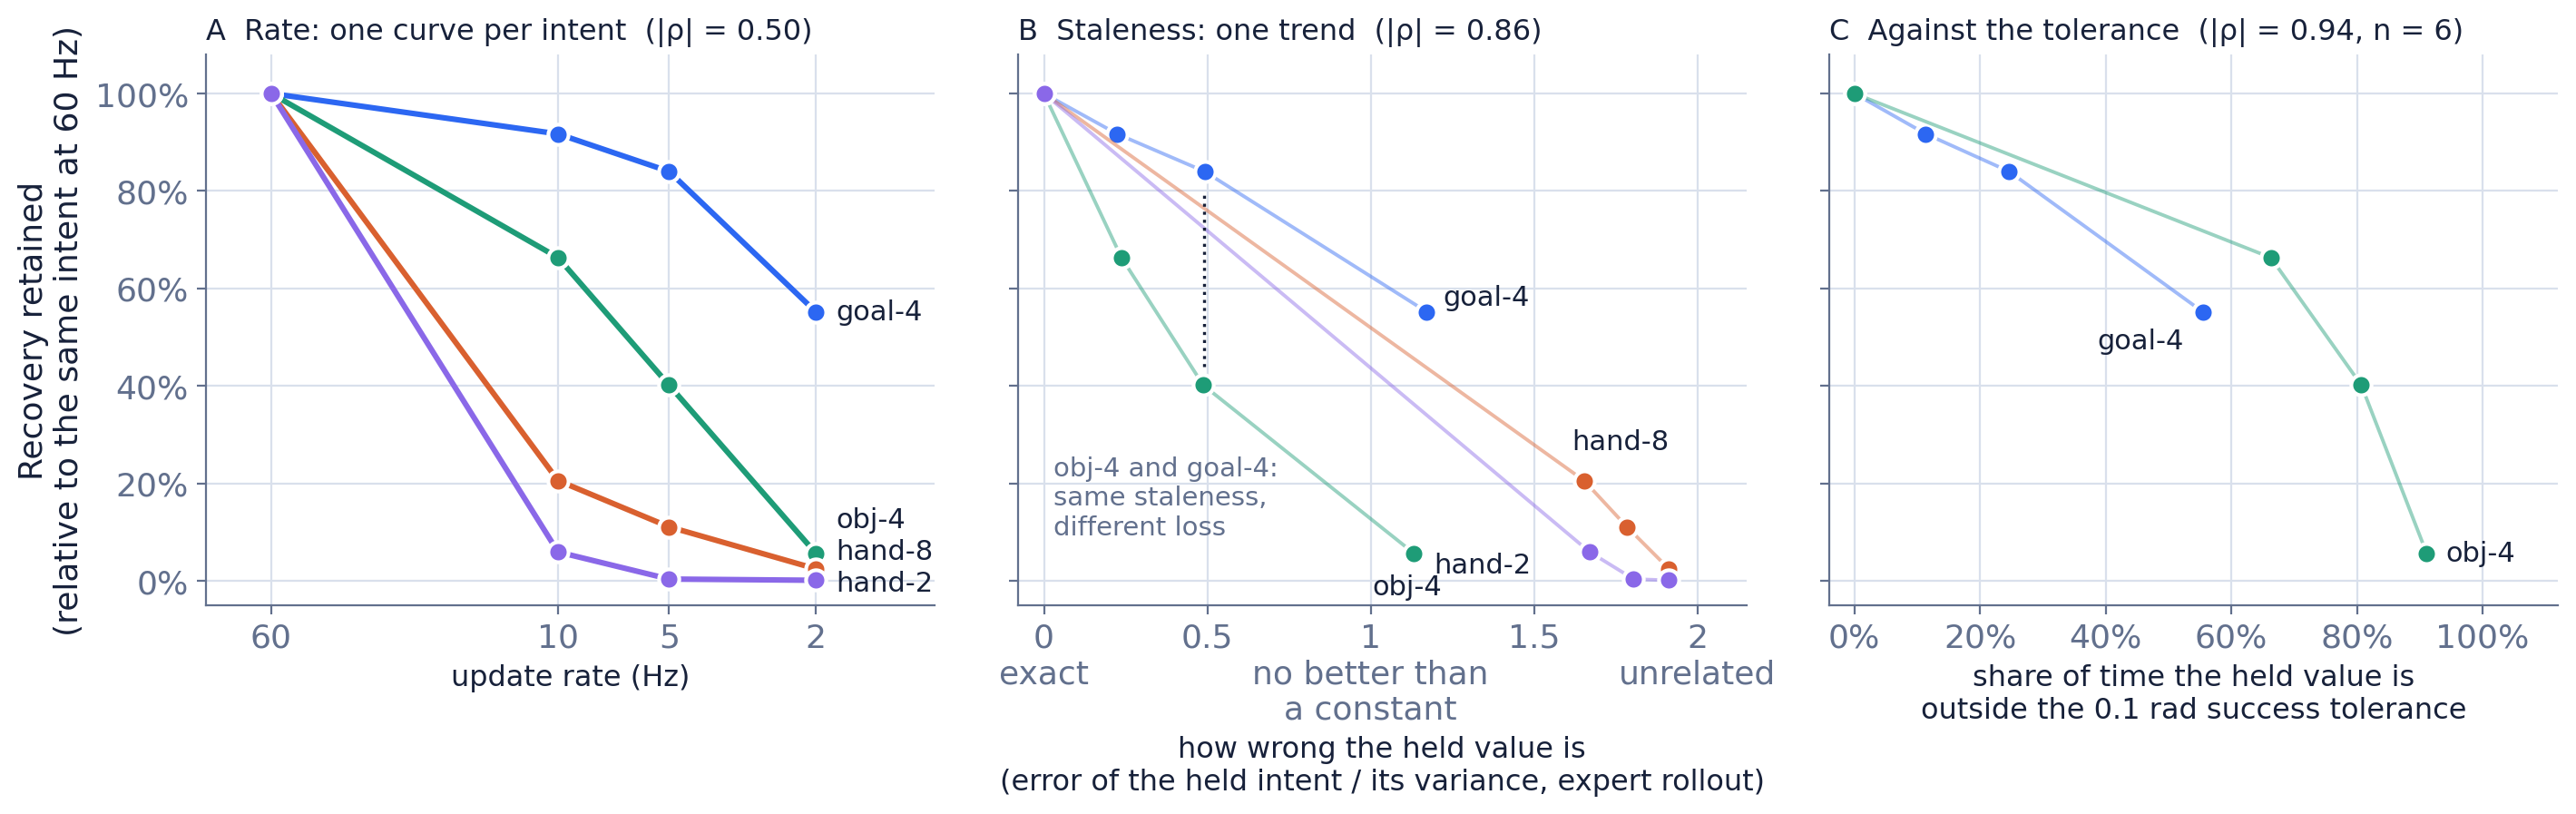
\includegraphics[width=\linewidth]{figures/staleness.png}
  \caption{Unified inter-update staleness collapse on Task~1. Plotting retained recovery against update rate (A) yields separate curves per interface ($|\rho|=0.50$), whereas plotting against normalized inter-update staleness (B, $|\rho|=0.86$) and fraction of steps outside the 0.1~rad success tolerance (C, $|\rho|=0.94$) collapses all interfaces onto a single monotonic trend.}
  \label{fig:app_staleness}
\end{figure}

\paragraph{E3 \texttt{any}-goal diagnostics.}
On \texttt{Unified v4}, masking \texttt{obs[68:72]} (relative rotation) drops the frozen teacher's \texttt{any}/\texttt{up} throughput from 29.4/50.0 to 0.03, whereas masking the goal quaternion alone keeps 25.3/45.8.
Removing the 120-step timeout (V1) still fails to learn \texttt{any} (0.003--0.028), while training \texttt{any}-only with timeout (V2) succeeds (3.0--4.6), implicating mixed-goal interference.
Appending \texttt{obs[68:72]} (\texttt{goal-11}, 6 seeds) yields 2/6 seeds learning \texttt{any} (vs.\ 0/6 for \texttt{goal-7}, Fisher one-sided $p=0.23$) and significantly higher \texttt{up} completions (15.1--31.1 vs.\ 8.1--14.8, MWU $p=0.002$, Welch $p=0.029$).

\section{Complete Scheme C Perception, Benchmark, and Open-Loop Audit Tables}
\label{app:scheme_c}

\begin{table}[h]
  \centering
  \caption{Held-out Z1 180-frame perception and overfitting-boundary audit (\texttt{test} split, 3-view \texttt{montage}, zero SoM tags, CircularEval). \texttt{C1-v1} generalizes visually; \texttt{C1-v2} repairs abstention (CBD) and unseen prompt \texttt{v3}.}
  \label{tab:vlm_perception}
  \small
  \setlength{\tabcolsep}{4.5pt}
  \resizebox{\linewidth}{!}{%
  \begin{tabular}{lcccccc}
    \toprule
    Model & Canonical All/\texttt{band} & \texttt{@nohand} & OOD G$\leftrightarrow$B & Novel Palette \texttt{band} & Unseen \texttt{v3} All/\texttt{turned} & Unans.\ CBD ($n=21$) \\
    \midrule
    Zero-shot \texttt{Qwen3-VL-8B} & --- / 7.5\% & --- / 5.7\% & --- & --- & --- & 52.4\% \\
    \texttt{C1-v1} (2 ep, Map-then-Reason) & \textbf{99.4} / \textbf{99.4\%} & \textbf{99.4\%} & \textbf{96.2\%} & 89.9\% & 36.8 / 60.0\% & 0.0\% \\
    \textbf{\texttt{C1-v2}} (1 ep, +CBD/+tpl/+CoT) & 98.7 / 98.7\% & 96.9\% & \textbf{96.2\%} & \textbf{93.7\%} & \textbf{59.2} / \textbf{96.7\%} & \textbf{100.0\%} \\
    \bottomrule
  \end{tabular}%
  }
\end{table}

\begin{table}[h]
  \centering
  \caption{Zero-shot Z1 visual-mode ablation on \texttt{Qwen3-VL-8B-Instruct} (180 \texttt{test} frames, \texttt{c1+s040+s220}, CircularEval; vanilla in parentheses). Only Set-of-Mark (\texttt{som}) unlocks \texttt{band} zero-shot, proving spatial grounding is the bottleneck.}
  \label{tab:app_z1_modes}
  \small
  \begin{tabular}{lccccc}
    \toprule
    Question & \texttt{raw} & \texttt{crop} & \texttt{montage} & \texttt{seam} & \texttt{som} \\
    \midrule
    \texttt{up} & 0.806 (0.928) & 0.861 (0.967) & \textbf{0.900} (0.939) & 0.878 (0.967) & 0.867 (0.961) \\
    \texttt{turned} & 0.178 (0.517) & 0.100 (0.633) & 0.311 (0.689) & 0.228 (0.706) & \textbf{0.800} (0.800) \\
    \texttt{band} ($n=159$) & 0.069 (0.226) & 0.031 (0.239) & 0.075 (0.151) & 0.075 (0.195) & \textbf{0.679} (0.792) \\
    \texttt{all\_levels} & 0.000 & 0.000 & 0.000 & 0.025 & \textbf{0.509} \\
    \bottomrule
  \end{tabular}
\end{table}

\begin{table}[h]
  \centering
  \caption{Public spatial benchmark retention after frozen-ViT LoRA SFT (\texttt{C1-v1}, Job \texttt{1175804}) vs.\ base \texttt{Qwen3-VL-8B-Instruct} (Job \texttt{1166604}). Truncation drops from 6.6--7.8\% to 0.0\%.}
  \label{tab:app_public_bench}
  \small
  \resizebox{\linewidth}{!}{%
  \begin{tabular}{lrrrr}
    \toprule
    Benchmark (Questions) & Base Greedy / Qwen & \texttt{C1-v1} Greedy / Qwen & $\Delta$ (Greedy / Qwen) & Mean Tokens (Base $\to$ SFT) \\
    \midrule
    EmbSpatial (3,640) & 78.24\% / 78.38\% & \textbf{76.35\%} / \textbf{76.43\%} & $-1.89\%$ / $-1.95\%$ & $9.5 \to 9.6$ \\
    MMStar (1,500) & 67.87\% / 69.27\% & \textbf{66.73\%} / \textbf{67.33\%} & $-1.13\%$ / $-1.93\%$ & $479.9 \to 6.1$ \\
    BLINK (1,901) & 67.02\% / 66.91\% & \textbf{63.18\%} / \textbf{62.70\%} & $-3.84\%$ / $-4.21\%$ & $357.7 \to 5.1$ \\
    \bottomrule
  \end{tabular}%
  }
\end{table}

\begin{table}[h]
  \centering
  \caption{Open-loop 96-state perception ($n=180$) and BFS macro-action optimality ($n=360$, $L=1..4$) across Scheme C variants. Unseen-camera \texttt{C1-v1} perception: \texttt{c1} 96.1\%, \texttt{s040+s220} 96.8\%, \texttt{s130+top} (unseen) 83.3\%, \texttt{top} 47.1\%.}
  \label{tab:app_openloop}
  \small
  \resizebox{\linewidth}{!}{%
  \begin{tabular}{lcccccc}
    \toprule
    Model & 96-State Can./OOD & Action Opt. & \texttt{reorient} ($n=264$) & \texttt{turn} ($n=96$) & $L1/L2/L3/L4$ Opt. \\
    \midrule
    \texttt{color\_invariant} (no plan SFT) & 71.7\% / 65.0\% & 0.0\% & 0.0\% & 0.0\% & --- \\
    \texttt{C1-v1} (\texttt{vision\_full}) & 87.2\% / \textbf{90.0\%} & 93.1\% & \textbf{98.9\%} & 77.1\% & 98.0 / 79.8 / 99.0 / \textbf{100.0\%} \\
    \texttt{C2-Grounded} GRPO & 88.3\% / 88.9\% & 92.8\% & 98.5\% & 77.1\% & 97.0 / 79.8 / 99.0 / \textbf{100.0\%} \\
    \texttt{C2-Terminal} GRPO & 87.8\% / \textbf{90.0\%} & 93.1\% & \textbf{98.9\%} & 77.1\% & 98.0 / 79.8 / 99.0 / \textbf{100.0\%} \\
    \textbf{\texttt{C1-v2} (cyclic turn CoT)} & \textbf{88.9\%} / 87.2\% & \textbf{96.1\%} & 98.5\% & \textbf{89.6\%} & 97.0 / \textbf{91.7} / \textbf{100.0} / 96.2\% \\
    \bottomrule
  \end{tabular}%
  }
\end{table}

\begin{table}[h]
  \centering
  \caption{Zero-shot 60~Hz Isaac Lab closed-loop generalization suite for \texttt{C1-v2} over frozen \texttt{Unified v4} (Jobs~\texttt{1177273}, \texttt{1177367}, \texttt{1177677}, \texttt{1177987}).}
  \label{tab:app_cl_gen}
  \small
  \resizebox{\linewidth}{!}{%
  \begin{tabular}{lcccc}
    \toprule
    Zero-Shot Perturbation & Protocol & Physical Success & Live 96-State Acc. & Key Finding / Failure Mode \\
    \midrule
    10$\times$ dark low-light (\texttt{intensity=200}) & 32 eps ($L{=}1..4$) & \textbf{100.0\%} (32/32) & \textbf{100.0\%} (80/80) & 1.000$\times$ optimal rounds, 0\% drops \\
    Warm-dim (\texttt{650}) / cool-bright (\texttt{3400}) & Demo episodes & \textbf{100.0\%} & \textbf{100.0\%} & Optimal rounds, 0\% drops \\
    OOD G$\leftrightarrow$B swapped cube (USD shader) & Demo episode & \textbf{100.0\%} (3/3 rds) & \textbf{100.0\%} & Optimal rounds, 0\% drops \\
    Pure casual prompt (no Map-then-Reason) & 32 eps ($L{=}1..4$) & 18.8\% (6/32) & 0.0\% & $L{=}1$: 75\% (6/8); $L{\ge}2$: 0\% (skips map) \\
    Novel palette (\texttt{orange/cyan/purple/pink}) & Demo episode & 0.0\% & 0.0\% & Perception 93.7\%, but pink$\leftrightarrow$white \& canonical CoT \\
    \bottomrule
  \end{tabular}%
  }
\end{table}
